\documentclass[runningheads]{llncs}

\usepackage[T1]{fontenc}
\usepackage{graphicx}
\usepackage{amsmath,amssymb,amsfonts}
\usepackage{booktabs}
\usepackage{algorithm}
\usepackage{algorithmic}
\usepackage{hyperref}
\usepackage{url}

\begin{document}

\title{An Intelligent System for Resilient Municipal Waste Governance: Heuristic-Guided Deep Reinforcement Learning over an Agent-Based Behavioral Model}

\author{X}
\authorrunning{X}

\institute{X}

\maketitle              

\begin{abstract}
Effective municipal solid waste (MSW) segregation is a critical sustainability bottleneck in developing urban centers. This implementation gap is exemplified by the ``MRF Paradox''---a scenario where localized increases in waste infrastructure are countered by a concurrent surge in illegal dumping. Standard Deep Reinforcement Learning (DRL) fails to resolve this via policy optimization due to the sparse reward problem caused by cultural behavioral inertia. To address this, we introduce a socio-technical framework coupling an Agent-Based Model (ABM) with a Heuristic-Guided DRL (HuDRL) agent for predictive governance. Using a local municipality as a testbed, household cognition is modeled via the Theory of Planned Behavior (TPB). Global Sensitivity Analysis proves that internal household friction is the dominant driver of non-compliance, accounting for 79\% of system variance. To navigate this non-convex policy space, our MDP utilizes action masking and heuristic guardrails. Simulations reveal that while standard policies stagnate, HuDRL converges on a ``Sequential Saturation'' strategy---concentrating funding into single nodes to trigger localized social tipping points. This approach establishes a mathematical framework for algorithmic governance and the optimization of limited public funds.

\keywords{Agent-Based Modeling \and Deep Reinforcement Learning \and Smart Cities \and Environmental Informatics \and Sustainable Urban Solutions \and Theory of Planned Behavior.}
\end{abstract}

\section{Introduction}
In the Philippines, despite the strict mandates of R.A. 9003 [1], a systemic implementation gap known as the ``MRF Paradox'' persists: while mandated Material Recovery Facilities (MRFs) increased by 8.7\% between 2023 and 2024, illegal dumpsites concurrently surged by 84\% [14]. This indicates that infrastructure alone is insufficient to override deeply ingrained cultural non-compliance. Current municipal trial-and-error resource allocation is no longer fiscally viable; Local Government Units (LGUs) require advanced predictive analytics to operationalize accountability and justify expenditure.

\section{Related Work}
Designing cost-efficient policy requires psychological grounding. The Theory of Planned Behavior (TPB) posits intention as a function of Attitude, Norms, and Control [7], yet environmental compliance is frequently overridden by the ``Cost of Effort'' [12]. We distinguish between the lower tipping point ($\sim$25--40\%) required to trigger initial adoption cascades [3], and the higher threshold (70\%) at which conformity becomes a self-sustaining cultural lock-in [4]. We implement the latter as the ``Social Norm Shield.'' Traditional optimization fails to capture such non-linear social hysteresis [2], but MDP-based neural networks can discover adaptive strategies via action masking [8].

\section{The Multi-Agent Environment}
\subsection{Household Agents and Cognitive Logic}
Household agents operate as continuous finite state machines. Their cognition is governed by a dynamically weighted TPB utility equation [63]:
\begin{equation}
U_{seg} = (w_{A}(t)A) + (w_{SN}(t)SN_{loc}) + (w_{PBC}(t)PBC) - C_{Net} + \epsilon
\end{equation}
The simulation incorporates a ``Bayanihan'' transitional state, establishing a 40\% compliance floor ($SN_{loc} \leftarrow \max(SN_{raw}, 0.40)$) [77]. This represents a psychological floor where motivation is sustained by community reciprocity.

\section{Deep Reinforcement Learning Agent}
The central policymaker is formalized as an episodic MDP. The Actor outputs the mean of a Gaussian policy with learned log-standard deviation; actions are sampled and mapped to the probability simplex $\Delta^{20}$ via a modified Softmax function [98]. To solve the sparse reward problem [8], we utilize a composite reward function:
\begin{equation}
R_{t} = \omega_{1}R_{Base} + \omega_{2}R_{Jackpot} + \omega_{3}R_{Focus} - \omega_{4}P_{Waste} + \Phi_{cap}
\end{equation}
To ensure training stability, the agent is constrained by heuristic guardrails, including a ``Phase-Shift Crisis Guardrail'' that forces 50\% of the budget to the weakest locale if global compliance falls below 40\% [114].

\section{Results and Discussion}
HuDRL achieved a mean reward of 10554.99 with low variance ($\sigma=4.02$) [148]. As shown in Fig. 1, HuDRL exhibits stable convergence, whereas Vanilla PPO remains trapped in the ``Collapse Zone'' [132]. Simulations reveal that HuDRL autonomously executed a ``Sequential Saturation'' strategy, concentrating up to 69\% of funds on specific urban bottlenecks to trigger habit internalization [163].

\begin{figure}
\centering
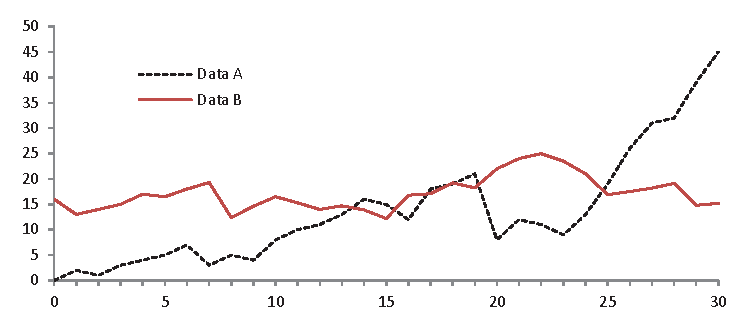
\includegraphics[width=0.7\textwidth]{fig1.eps}
\caption{Training convergence curves demonstrating HuDRL's stable ascent compared to Vanilla PPO's stagnation.} \label{fig1}
\end{figure}

\section{Conclusion}
This study validates that coupling ABM with HuDRL provides a mathematically rigorous laboratory for policy optimization. The framework proves that overcoming household segregation friction requires targeted, sequential resource saturation [187]. Future research will explore transitioning this into a Municipal Digital Twin.

\subsubsection{Acknowledgements} 
The authors thank the local government units and the university department for providing essential data and support. Source code: \url{https://github.com/X/X}. During preparation, Gemini Pro was used solely for grammatical refinement. All technical content, equations, and algorithms were verified by the authors.

\begin{thebibliography}{8}
\bibitem{ref1} Rep. Act No. 9003, Philippines (2001)
\bibitem{ref2} Tian, X., et al.: Agent-based modeling in solid waste management. Env. Impact Assess. Rev. \textbf{110}, 107723 (2024)
\bibitem{ref3} Centola, D., et al.: Tipping points in social convention. Science \textbf{360}(6393), 1116--1119 (2018)
\bibitem{ref4} Nyborg, K., et al.: Social norms as solutions. Science \textbf{354}(6308), 42--43 (2016)
\bibitem{ref5} X, et al.: Knowledge, attitude, and practices on solid waste management (2025)
\bibitem{ref6} Zhao, A., et al.: Extrinsic incentives for rural waste sorting. Dev. Econ. \textbf{60}(3) (2022)
\bibitem{ref7} Taraghi, M., Yoder, L.: Theory of planned behavior in ABM. Ecol. Mod. \textbf{508}, 111231 (2025)
\bibitem{ref8} Zheng, S., et al.: The AI Economist. Science Adv. \textbf{8}(18) (2022)
\bibitem{ref12} Moeini, B., et al.: Household interventions for waste segregation. Sustainability \textbf{15}(24), 16546 (2023)
\bibitem{ref14} PSA: Compendium of Philippine Environment Statistics (2025)
\end{thebibliography}
\end{document}